\section{Results}\label{sec:results}
\begin{framed}
6. Implement and test a part of your system using the ZYBO platform including at least one IP core written and verified with the HLS tool.
\end{framed}

This section shows and elaborates on the results in performance and utilization of all the designs we purposed in section \ref{sec:archdesign}. This includes a high-level synthesis report of the two IP cores (GenerationGenerator and Simulator) and the user application, that was implemented in C++ and deployed to the ZYBO board with the use of OSAPI threads and FreeRTOS. Overall, our results show that simple fixed-point arithmetic can be accelerated in an hardware FPGA at relative low cost, however more complicated floating point computations are better done in software, as the number of required DSP's and lookup tables rapidly increase in such cases.

\subsection{HLS of the GenerationGenerator core}

The IP core was synthesized in C using a VivadoSimulator, a period of 20 and Verilog as the RTL language. Target device is a Zybo model xc7z010clg400-1. We used a SystemC stimuli file to invoke the IP core, which can be found in Appendix A. Figure \ref{fig:ggperformanceestimates} shows the performance estimates of the applied design. We seen that the estimated clock is well within our target of 20 with an uncertainty of 2.50 and the latency lie in range of 270 to 271.

\begin{figure}[htbp]
	\centering
	\fbox{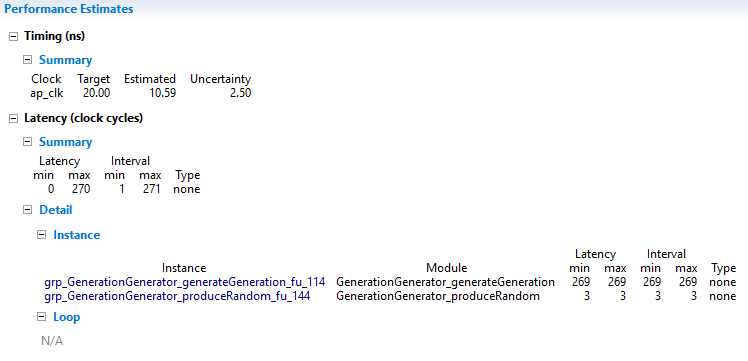
\includegraphics[width=1.0\linewidth]{../diagrams/GGperformanceEstimates.png}}
	\caption{X}
	\label{fig:ggperformanceestimates}
\end{figure}

Figure \ref{fig:ggutilizationestimates} shows utilization of hardware estimates. We see that the demand of resources are well within range of what is available on the Zybo board. 

\begin{figure}[htbp]
	\centering
	\fbox{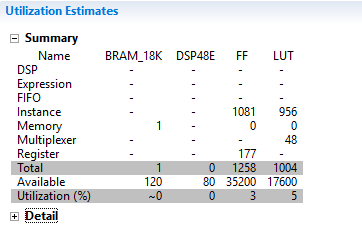
\includegraphics[width=1.0\linewidth]{../diagrams/GGutilizationEstimates.png}}
	\caption{X}
	\label{fig:ggutilizationestimates}
\end{figure}

Figure \ref{fig:gginterface} shows the generated interface signals. These echo the interfaces we defined in the definition of source file. Direction indicate if they are to be read or written to. The bit length stems from the width of a chromosome.

\begin{figure}[htbp]
	\centering
	\fbox{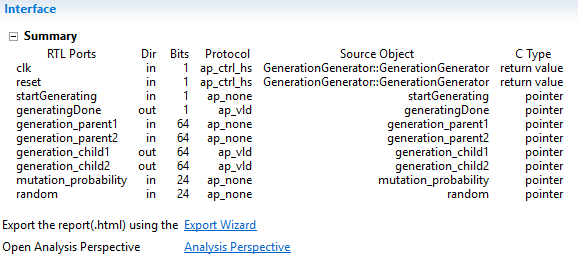
\includegraphics[width=1.0\linewidth]{../diagrams/GGinterface}}
	\caption{}
	\label{fig:gginterface}
\end{figure}

Figure \ref{fig:generationgeneratortrace} shows the trace output after running a simulation with a stimuli. We seen that the random input data changes continually, and when the generating core is started, it uses the two parents and a mutation probability to create new children chromosomes and output these.

\begin{figure}[htbp]
	\centering
	\fbox{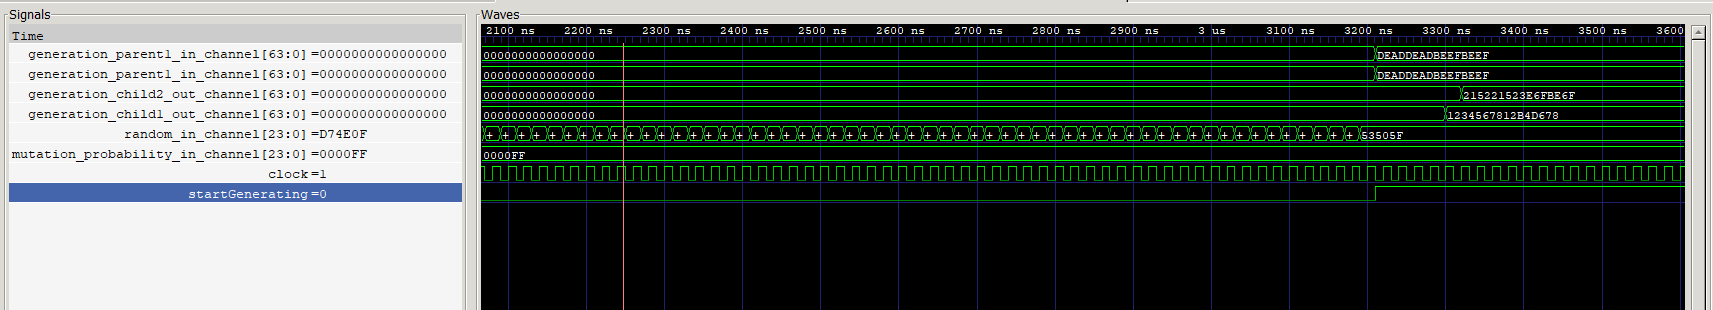
\includegraphics[width=1\linewidth]{../diagrams/GenerationGeneratorSim.png}}
	\caption{A trace diagram that shows all bidirectional signals of the module during a example stimulation.}
	\label{fig:generationgeneratortrace}
\end{figure}

\subsection{HLS of the Simulator core}

The IP was synthesized with the same settings as the GenerationGenertor in the Vivado HLS tool. We used a SystemC stimuli file to make calls to the IP core, which can be found in Appendix A. Figure \ref{fig:simperformanceestimates} shows performance estimates, with the estimated clock being within the range of the target clock and the latency being from  0 to 96. 

\begin{figure}[htbp]
	\centering
	\fbox{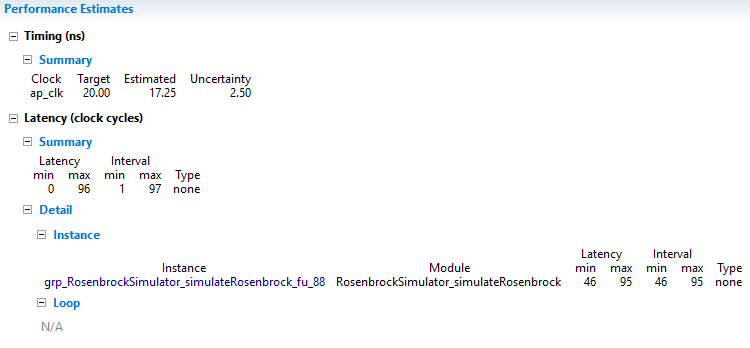
\includegraphics[width=1.0\linewidth]{../diagrams/SimperformanceEstimates.png}}
	\caption{X}
	\label{fig:simperformanceestimates}
\end{figure}

In figure \ref{fig:ggutilizationestimates} we see the utilization estimates of running the simulation in hardware. The total resource demand exceed those of the platform, the Zybo board, by quite a significant margin. The algorithm need 592 DSP48E's, but only 80 are available. Likewise it needs 39988 flip-flops and 22918 lookup tables, but fewer are available. This means that the current implementation will not be runnable on hardware.

\begin{figure}[htbp]
	\centering
	\fbox{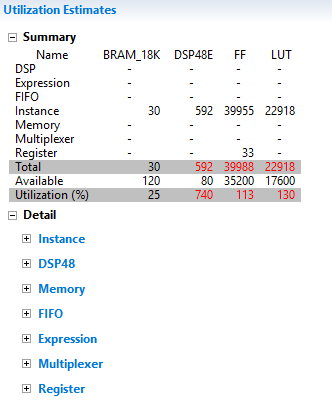
\includegraphics[width=1.0\linewidth]{../diagrams/SimutilizationEstimates.png}}
	\caption{X}
	\label{fig:simutilizationestimates}
\end{figure}

Figure \ref{fig:siminterface} shows the generated interface signals with the RTL ports and their respective direction and bit length. 

\begin{figure}[htbp]
	\centering
	\fbox{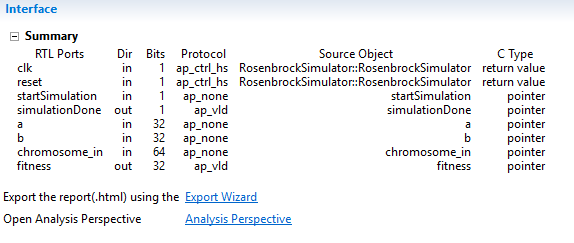
\includegraphics[width=1.0\linewidth]{../diagrams/Siminterface}}
	\caption{X}
	\label{fig:siminterface}
\end{figure}}
